%%%%%%%%%%%%%%%%%%%%%%%%%%%%%%%%%%%%%%%%%%%%%%%%%%%%%%%%
% Este é um documento que servirá de modelo para
% os relatórios feitos na disciplina Circuitos Digitais
% 2016-2
%%%%%%%%%%%%%%%%%%%%%%%%%%%%%%%%%%%%%%%%%%%%%%%%%%%%%%%%%

\PassOptionsToPackage{brazil,american}{babel}
\documentclass[12pt]{article}

\usepackage{sbc-template}
\usepackage[brazil,american]{babel}
\usepackage[utf8]{inputenc}

\usepackage{graphicx}
\usepackage{url}
\usepackage{float}
\usepackage{listings}
\usepackage{color}
\usepackage{todonotes}
\usepackage{algorithmic}
\usepackage{algorithm}
\usepackage{hyperref}
     
\sloppy

\title{Experimento 5\\ 
	Circuitos Combinacionais: Codificador e Decodificador}

\author{
	Lucas Mafra Chagas, 12/0126443 \\
	Marcelo Giordano Martins Costa de Oliveira,  12/0037301
}


\address{Dep. Ciência da Computação -- Universidade de Brasília (UnB)\\
	CiC 116351 - Circuistos Digitais - Turma C
	\email{\{giordano.marcelo, chagas.lucas.mafra\}@gmail.com}
}

\begin{document} 

\maketitle

 \begin{abstract}
   Write here a short summary of the report in English. This corresponds to the Experiment 7 report on combinational circuits, specifically the multiplexers.
 \end{abstract}
     
 \begin{resumo} 
  Escreva aqui um pequeno resumo do relatório. Este corresponde ao relatório do Experimento 7 sobre circuitos combinacionais, especificamente os multiplexadores.
 \end{resumo}


\section{Objetivos}
\label{sec:Objetivos}

Elaboração de um codificador e de um decodificador usando-se circuitos combinacionais e
aplicando-se as técnicas de minimização de funções lógicas. Verificação da possibilidade
de conversão de um número decimal em um número binário de código qualquer e sua
posterior decodificação.

\section{Materiais} 
\label{sec:Materiais}

\begin{itemize}
    \item Software Quartus II versão 13.0
	\item Kit de desenvolvimento em FPGA DE2 Altera
    
\end{itemize}


\section{Introdução}
\label{sec:Introducao}

Os computadores são máquinas que trabalham com a utilização de um sistema binário para analisar variáveis e realizar cálculos. Já o homem está acostumado a raciocinar e trabalhar com o sistema decimal. Portanto, para que a comunicação homem-máquina possa ser feita de maneira mais direta, sem que o homem precise aprender a interpretar números binários, convém incorporar aos equipamentos de entrada e saída de computadores conversores de código decimal-binário e binário-decimal, respectivamente. Para o primeiro caso(onde a entrada é um número decimal), temos que o conversor é chamado de codificador, enquanto para o segundo caso (onde a saída é um número decimal) ele é chamado de decodificador.

\begin{figure}[H]
	\centering
	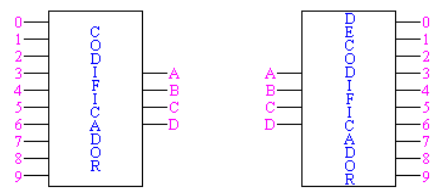
\includegraphics[width=.5\textwidth]{coddecod.jpg}
	\caption{Codificador e Decodificador.}
	\label{fig:coddecod}
\end{figure}


Para o codificador, teremos uma, e somente uma, entrada ativada a cada instante. A saída corresponderá à forma codificada desse decimal (utilizando apenas 0’s e 1’s). Já para o decodificador, temos que todas as entradas são ativadas no mesmo instante, porém, elas geram apenas uma saída. 
Para este experimento, será criado um codificafor decimal-Código de Gray e um decodificador Código de Gray-binário. Este código é determinado como apresenta a tabela abaixo:

\begin{table}[H]
	\centering
	\begin{tabular}{|c|c|c|c|c|}
		\cline{1-5}
		\multicolumn{1}{|c|}{Decimal} & \multicolumn{1}{|c|}{A} & \multicolumn{1}{|c|}{B} & \multicolumn{1}{|c|}{C} & \multicolumn{1}{|c|}{D}\\
		\hline
		0 & 0 & 0 & 0 & 0 \\
		\hline
		1 & 0 & 0 & 0 & 1 \\
		\hline
		2 & 0 & 0 & 1 & 1 \\
		\hline
		3 & 0 & 0 & 1 & 0 \\
		\hline
		4 & 0 & 1 & 1 & 0 \\
		\hline
		5 & 0 & 1 & 1 & 1 \\
		\hline
		6 & 0 & 1 & 0 & 1 \\
		\hline
		7 & 0 & 1 & 0 & 0 \\
		\hline
		8 & 1 & 1 & 0 & 0 \\
		\hline
		9 & 1 & 1 & 0 & 1 \\
		\hline
	\end{tabular}
	
\end{table} 




\section{Procedimentos}
\label{sec:Procedimentos}

Neste relatório, precisamos fazer:
\begin{itemize}
	\item Obter as funções booleanas para o codificador.
	\item Fazer simulações funcional e temporal do diagrama lógico do codificador no Quartus. 
	\item Obter as funções booleanas para o decodificador.
	\item Fazer simulações funcional e temporal do diagrama lógico do decodificador no Quartus. 
	\item Filmar o funcionamento do codificador e decodificador feito no Quartus II.
\end{itemize}

\subsection{Funções Booleanas para o Codificador}
\label{sec:Cod}


\begin{figure}[H]
	\centering
	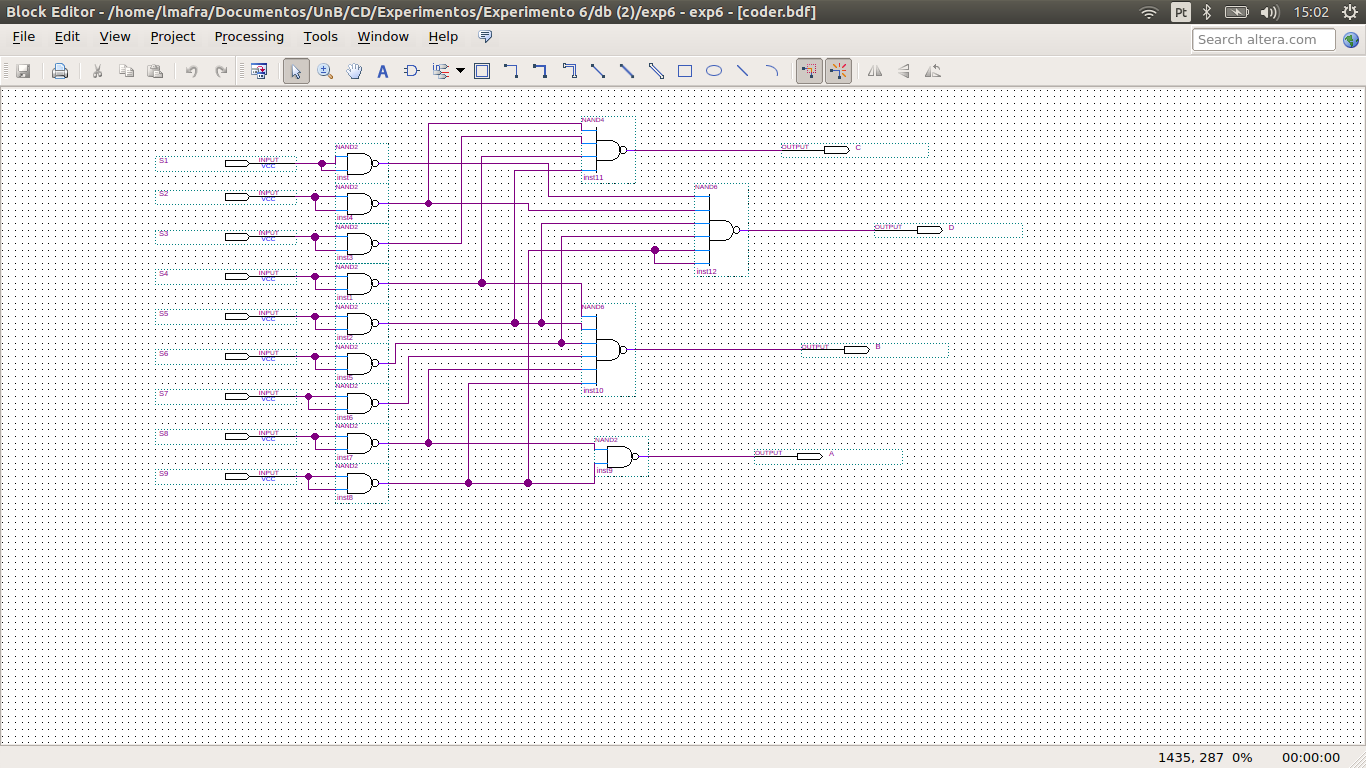
\includegraphics[width=1\textwidth]{coder.png}
	\caption{Codificador.}
	\label{fig:coder}
\end{figure}

\begin{figure}[H]
	\centering
	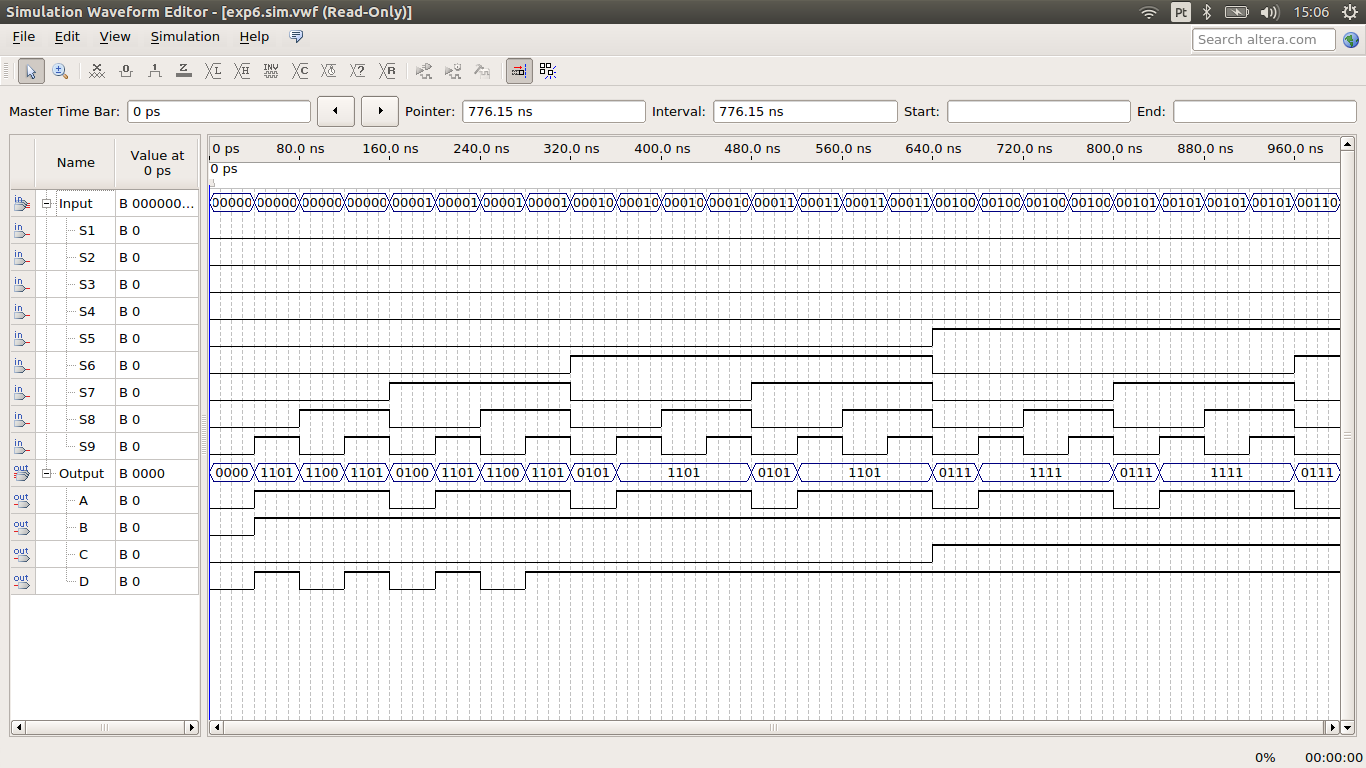
\includegraphics[width=1\textwidth]{functionalcoder.png}
	\caption{Simulação funcional do codificador.}
	\label{fig:funccoder}
\end{figure}

\begin{figure}[H]
	\centering
	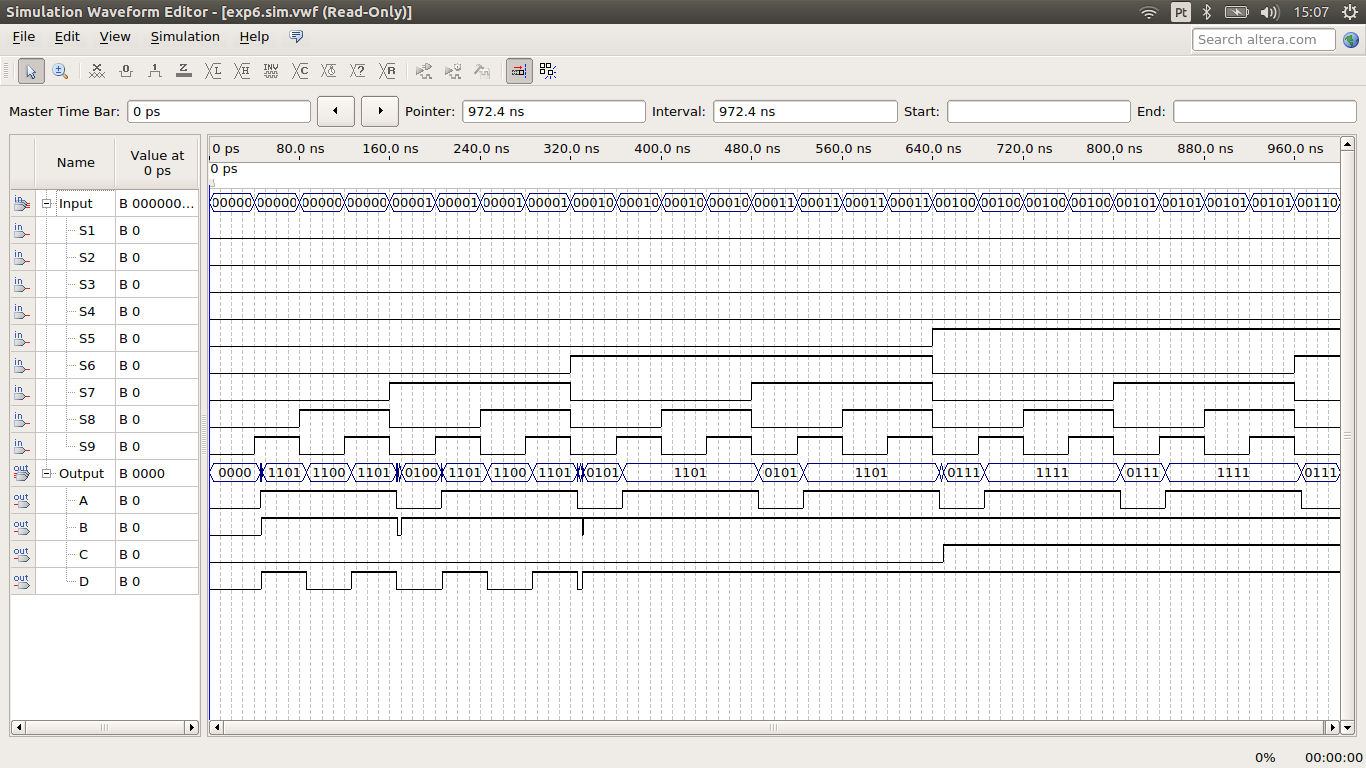
\includegraphics[width=1\textwidth]{timingcoder.png}
	\caption{Simulação temporal do codificador.}
	\label{fig:timecoder}
\end{figure}


\subsection{Funções Booleanas para o Decodificador}
\label{sec:Decod}

\begin{figure}[H]
	\centering
	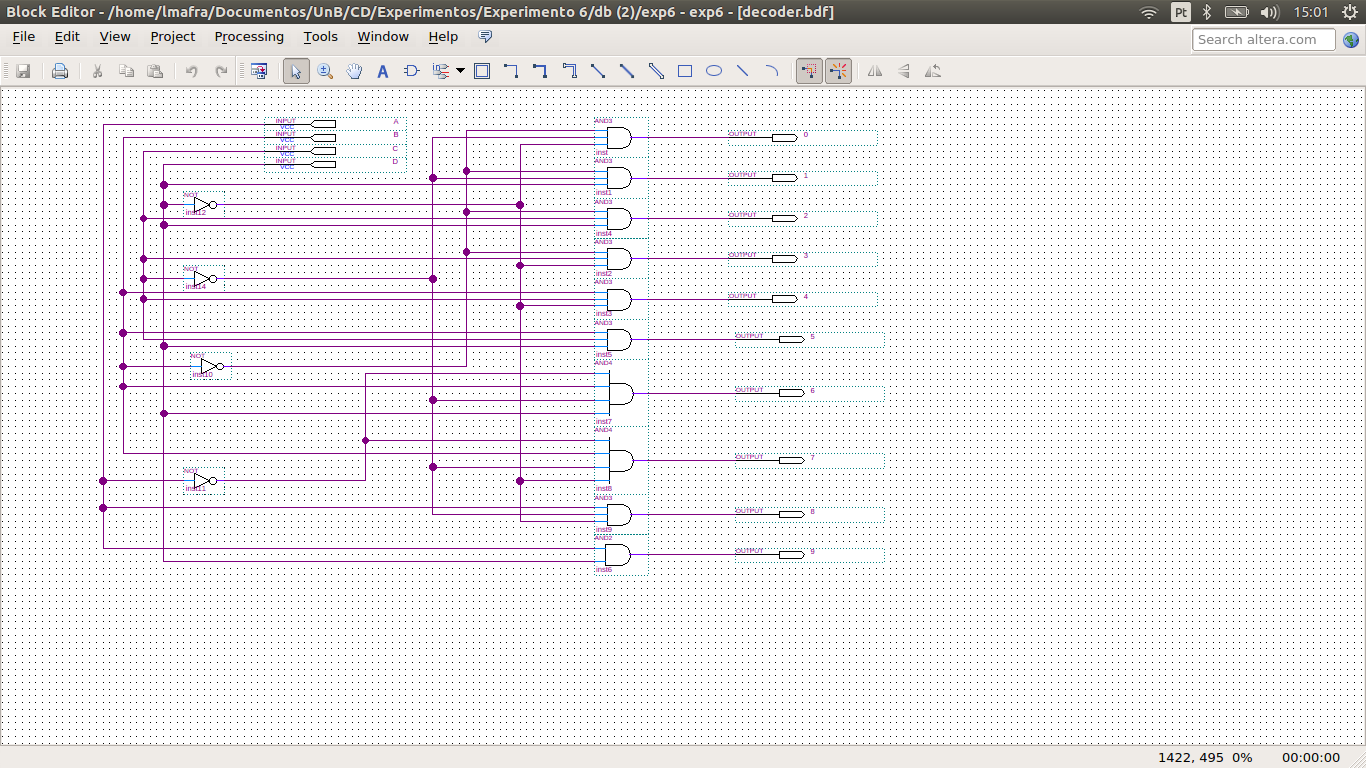
\includegraphics[width=1\textwidth]{decoder.png}
	\caption{Decodificador.}
	\label{fig:decoder}
\end{figure}

\begin{figure}[H]
	\centering
	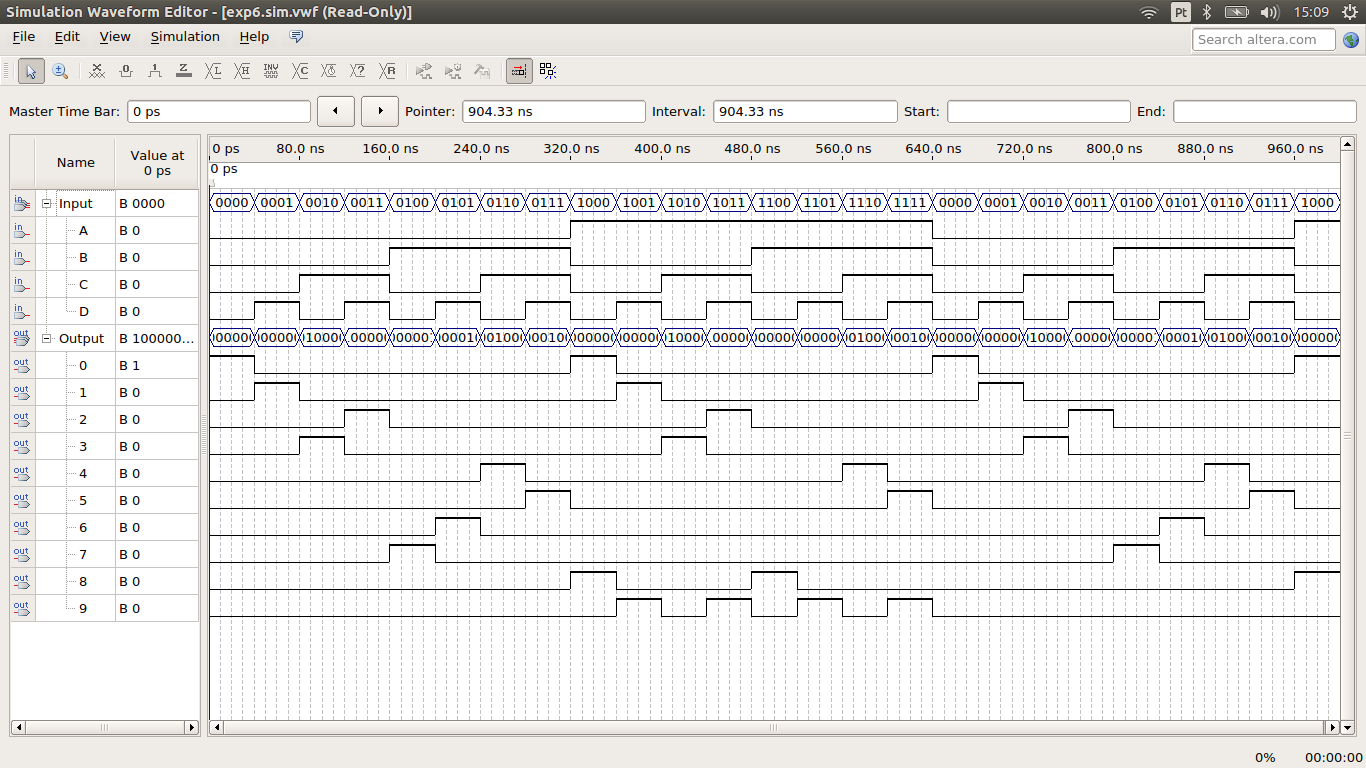
\includegraphics[width=1\textwidth]{functionaldecoder.png}
	\caption{Simulação funcional do decodificador.}
	\label{fig:funcdecoder}
\end{figure}

\begin{figure}[H]
	\centering
	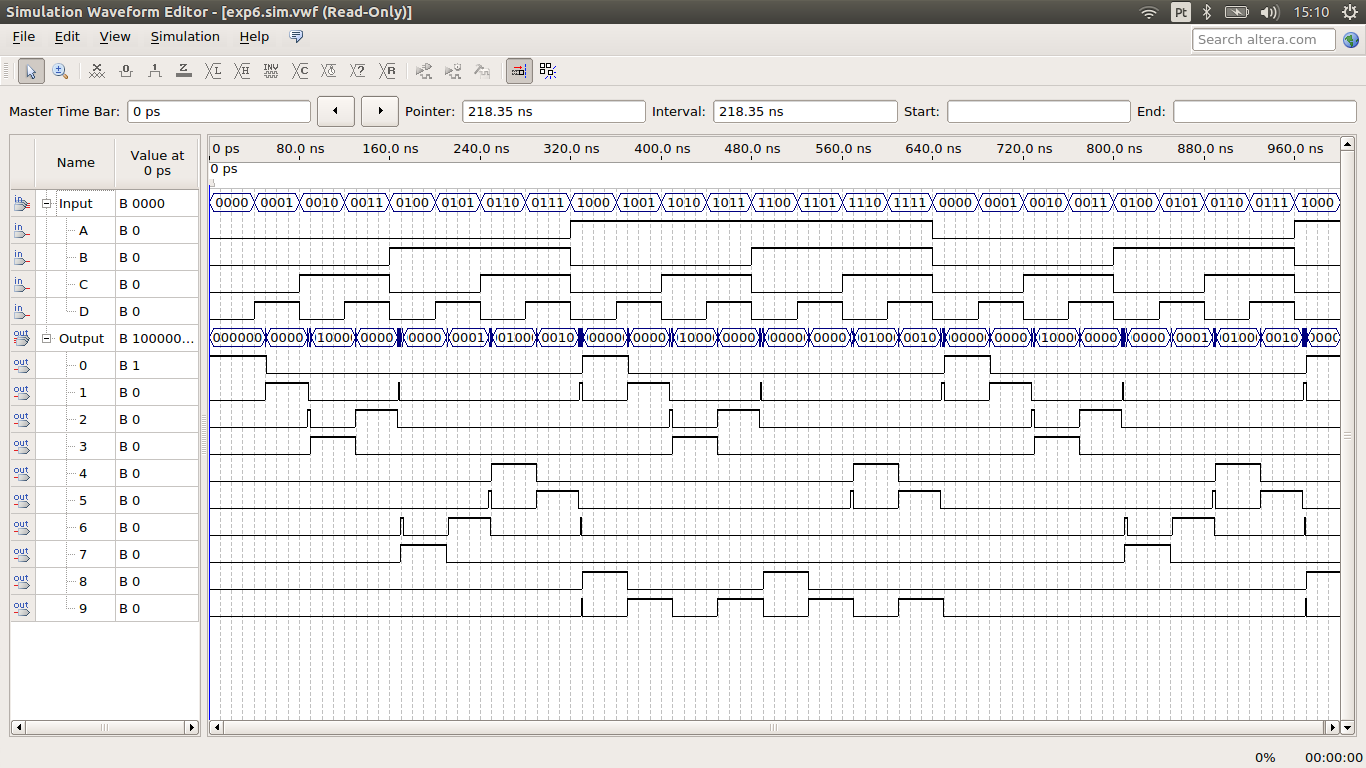
\includegraphics[width=1\textwidth]{timingdecoder.png}
	\caption{Simulação temporal do decodificador.}
	\label{fig:timedecoder}
\end{figure}

\subsection{Funcionamento do Codificador e Decodificador}

Desenvolvemos no kit de desenvolvimento em FPGA DE2 Altera o código projetado com o codificador e decodificador projetado na imagem abaixo. 

\begin{figure}[H]
	\centering
	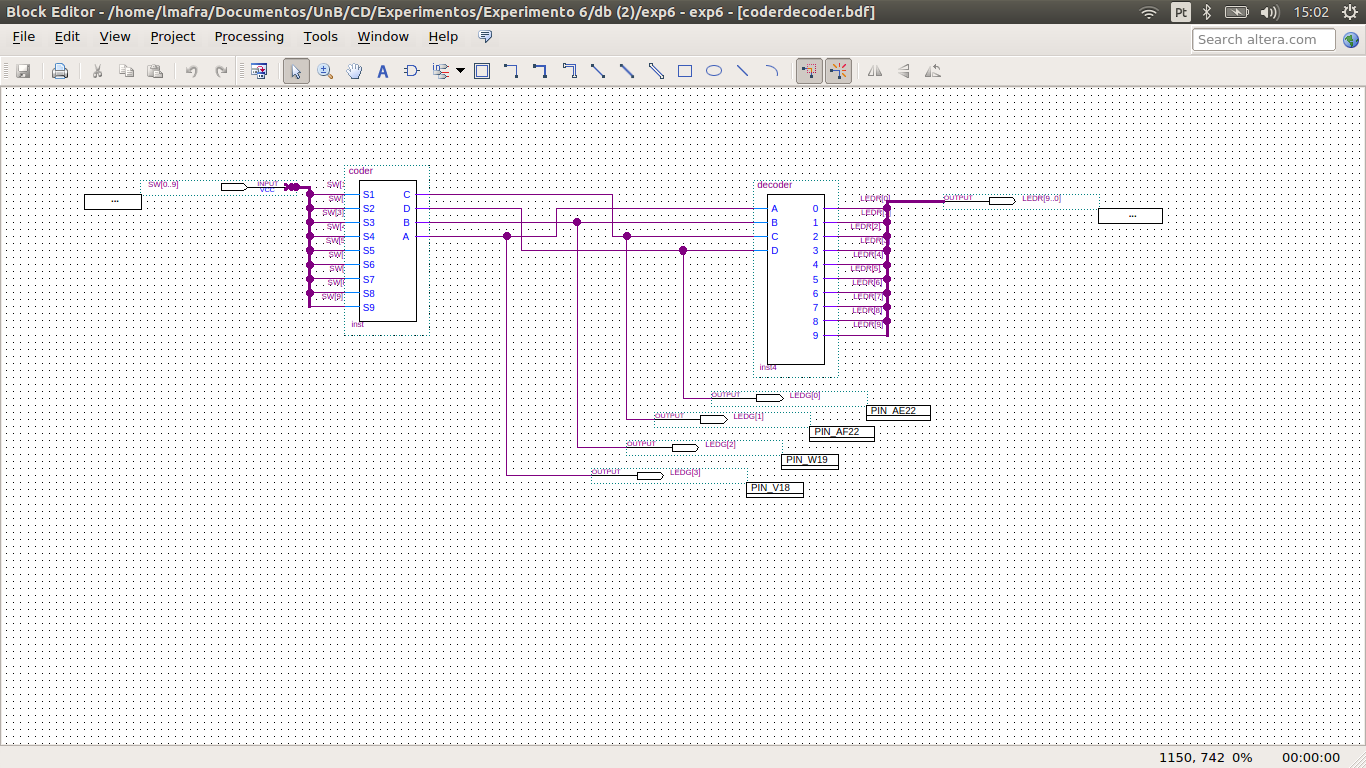
\includegraphics[width=1\textwidth]{coderdecoder.png}
	\caption{Circuito contendo codificador e decodificador.}
	\label{fig:coderdecoder}
\end{figure}

É possível ver o resultado no seguinte link: \href{https://www.youtube.com/watch?v=paRaiHqDqBo}{Vídeo no Youtube}


\section{Análise dos Resultados}
\label{sec:Resultados}

Faça uma análise crítica dos resultados obtidos nos experimentos. Esta análise pode ser feita item a item ou de uma forma geral.

Dica: Use pesquisa na Internet para tirar as dúvidas sobre edição em \LaTeX .

\section{Conclusão}
\label{sec:Conclusao}

A partir do experimento foi possível ampliar os conhecimentos sobre codificadores e decodificadores. A montagem desses circuitos aperfeiçoou ainda mais a já conhecida teoria a respeito deles. Circuitos simples como esses são bases para o avanço da tecnologia, e de toda essa gama de aparelhos que temos hoje, eles abrem portas para muitas possibilidades e a familiarização com eles é, naturalmente, muito importante.


\bibliographystyle{sbc}
\bibliography{relatorio}


\newpage 
% Colocar aqui apenas as respostas dos itens da Auto-Avaliação
\section*{Auto-Avaliação}

\begin{enumerate}
    \item a
    \item c
    \item b
    \item c
    \item d
    \item Porta NOT A defeituosa, sempre com nível 0 na saída.
    \item Porta NOT D defeituosa, sempre com nível 1 na saída. 
    \item Porta NOT A defeituosa, sempre com nível 1 na saída.
\end{enumerate}


\end{document}
